\usetikzlibrary{shapes.geometric, shapes.arrows, arrows.meta, positioning, fit, backgrounds, calc, shadows}

% 定义自定义颜色 (近似原图)
\definecolor{cBlue}{HTML}{2E75B6}
\definecolor{cBlueBg}{HTML}{DEEBF7}
\definecolor{cGreen}{HTML}{548235}
\definecolor{cGreenBg}{HTML}{E2EFDA}
\definecolor{cOrange}{HTML}{C65911}
\definecolor{cOrangeBg}{HTML}{FCE4D6}
\definecolor{cRed}{HTML}{C00000}
\definecolor{cRedBg}{HTML}{F8CECC}
\definecolor{cYellow}{HTML}{FFD966} % 高亮背景
\definecolor{cArrow}{HTML}{BF9000}  % 金色箭头
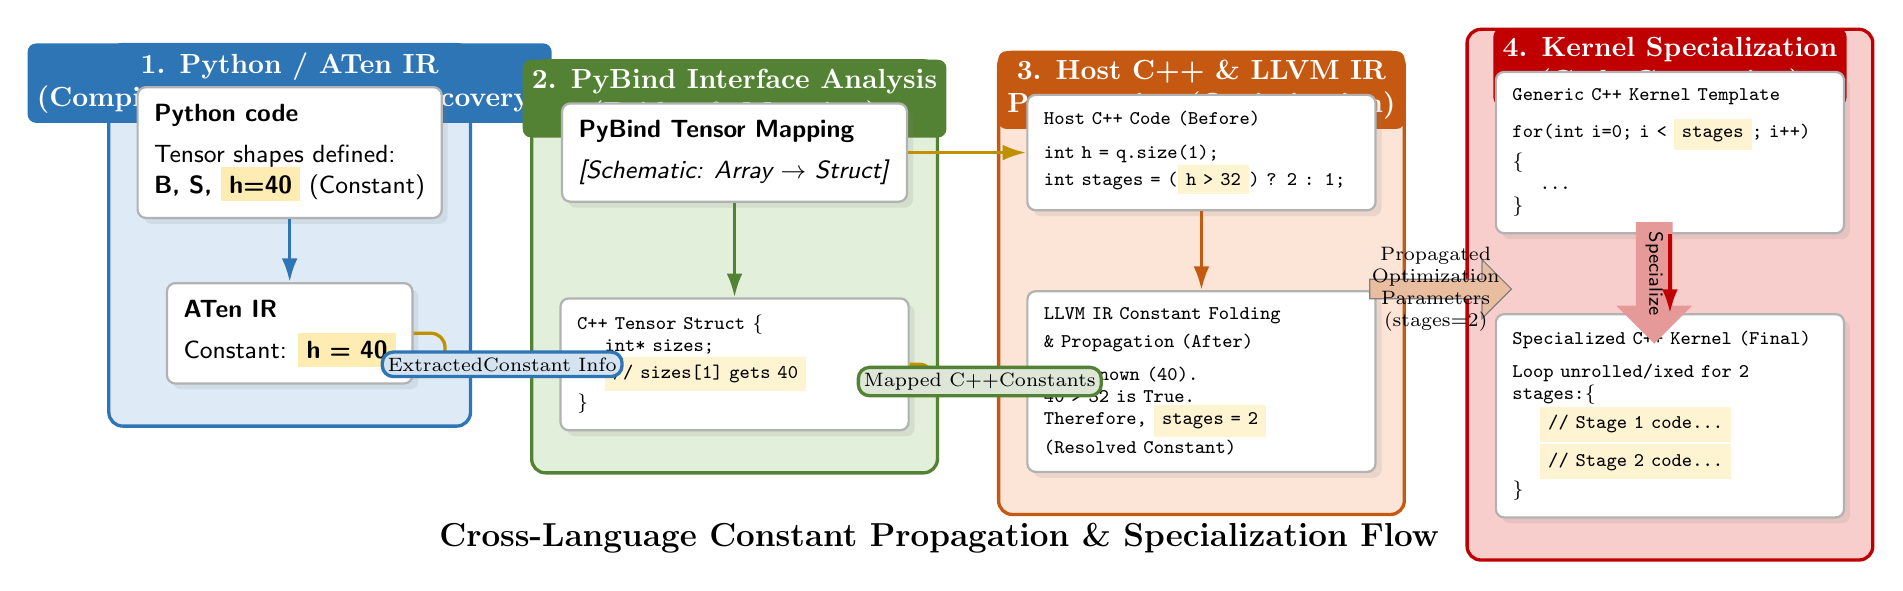
\begin{tikzpicture}[
    % 全局样式设置
    font=\sffamily\small,
    node distance=0.8cm and 0.6cm,
    % 内部代码块的样式
    codebox/.style={
        rectangle, 
        rounded corners=3pt, 
        draw=black!30, 
        thick, 
        fill=white, 
        align=left, 
        inner sep=6pt,
        drop shadow={opacity=0.15}
    },
    % 代码字体样式
    codefont/.style={
        font=\ttfamily\scriptsize,
        text width=4cm
    },
    % 每一列的大背景框样式
    colframe/.style 2 args={
        rectangle, 
        rounded corners=5pt, 
        draw=#1, 
        very thick, 
        fill=#2, 
        inner sep=10pt,
        inner ysep=15pt
    },
    % 标题样式
    header/.style={
        font=\bfseries\color{white},
        align=center,
        minimum height=2em
    },
    % 箭头样式
    flowarrow/.style={
        -{Latex[length=3mm, width=2mm]}, 
        very thick, 
        draw=black!70
    },
    constarrow/.style={
        -{Latex[length=3mm, width=2mm]}, 
        very thick, 
        draw=cArrow,
        rounded corners=5pt
    }
]

    % ==========================================
    % 第一列: Python / ATen IR (Blue)
    % ==========================================
    \node[codebox] (pycode) {
        \textbf{Python code}\\[4pt]
        Tensor shapes defined:\\
        \textbf{B, S, \colorbox{cYellow!50}{h=40}} (Constant)
    };
    
    \node[codebox, below=of pycode] (aten) {
        \textbf{ATen IR}\\[4pt]
        Constant: \colorbox{cYellow!50}{\textbf{h = 40}}
    };
    
    % 连接箭头
    \draw[flowarrow, cBlue] (pycode) -- (aten);

    % ==========================================
    % 第二列: PyBind Interface (Green)
    % ==========================================
    % 定位：在第一列右侧
    \node[codebox, right=1.5cm of pycode, anchor=west] (mapping) {
        \textbf{PyBind Tensor Mapping}\\[4pt]
        \textit{[Schematic: Array $\to$ Struct]}
    };

    \node[codebox, codefont, below=1.2cm of mapping] (cppstruct) {
        \textbf{C++ Tensor Struct \{}\\
        \hspace{1em} int* sizes;\\
        \hspace{1em} \colorbox{cYellow!30}{// sizes[1] gets 40}\\
        \}
    };

    % 连接箭头
    \draw[flowarrow, cGreen] (mapping) -- (cppstruct);

    % ==========================================
    % 第三列: Host C++ & LLVM IR (Orange)
    % ==========================================
    \node[codebox, codefont, right=1.5cm of mapping, anchor=west] (hostcpp) {
        \textbf{Host C++ Code (Before)}\\[4pt]
        int h = q.size(1);\\
        int stages = (\colorbox{cYellow!30}{h > 32}) ? 2 : 1;
    };

    \node[codebox, codefont, below=1.0cm of hostcpp] (llvm) {
        \textbf{LLVM IR Constant Folding}\\[2pt]
        \textbf{\& Propagation (After)}\\[4pt]
        \textbf{h} is known (40).\\
        40 > 32 is True.\\
        Therefore, \colorbox{cYellow!30}{\textbf{stages = 2}}\\
        (Resolved Constant)
    };
    
    % 连接箭头
    \draw[flowarrow, cOrange] (hostcpp) -- (llvm);

    % ==========================================
    % 第四列: Kernel Specialization (Red)
    % ==========================================
    \node[codebox, codefont, right=1.5cm of hostcpp, anchor=west] (template) {
        \textbf{Generic C++ Kernel Template}\\[4pt]
        for(int i=0; i < \colorbox{cYellow!30}{stages}; i++) \{\\
        \hspace{1em} ...\\
        \}
    };

    \node[codebox, codefont, below=1.0cm of template] (final) {
        \textbf{Specialized C++ Kernel (Final)}\\[4pt]
        Loop unrolled/ixed for 2 stages:\{\\
        \hspace{1em} \colorbox{cYellow!30}{// Stage 1 code...}\\
        \hspace{1em} \colorbox{cYellow!30}{// Stage 2 code...}\\
        \}
    };
    
    % 连接箭头 (宽箭头效果)
    \node[single arrow, draw=none, fill=cRed!40, minimum height=1cm, rotate=-90, yshift=-2mm] at ($(template.south)!0.5!(final.north)$) {\scriptsize Specialize};
    \draw[flowarrow, cRed] (template) -- (final);

    % ==========================================
    % 绘制背景框 (Fit Library)
    % ==========================================
    
    % Column 1 Background
    \begin{scope}[on background layer]
        \node[colframe={cBlue}{cBlueBg}, fit=(pycode)(aten)] (col1) {};
        \node[header, fill=cBlue, anchor=north, rounded corners=3pt] at (col1.north) {1. Python / ATen IR\\(Compile Time Constant Discovery)};
        
        % Column 2 Background
        \node[colframe={cGreen}{cGreenBg}, fit=(mapping)(cppstruct)] (col2) {};
        \node[header, fill=cGreen, anchor=north, rounded corners=3pt] at (col2.north) {2. PyBind Interface Analysis\\(Bridge \& Mapping)};

        % Column 3 Background
        \node[colframe={cOrange}{cOrangeBg}, fit=(hostcpp)(llvm)] (col3) {};
        \node[header, fill=cOrange, anchor=north, rounded corners=3pt] at (col3.north) {3. Host C++ \& LLVM IR\\Propagation (Optimization)};

        % Column 4 Background
        \node[colframe={cRed}{cRedBg}, fit=(template)(final)] (col4) {};
        \node[header, fill=cRed, anchor=north, rounded corners=3pt] at (col4.north) {4. Kernel Specialization\\(Code Generation)};
    \end{scope}

    % ==========================================
    % 跨列的复杂箭头 (Golden Arrows)
    % ==========================================

    % 1. ATen IR -> C++ Struct (Extracted Constant Info)
    \draw[constarrow] (aten.east) -- ++(0.4,0) |- (cppstruct.west) node[midway, fill=cBlue!20, draw=cBlue, text=black, font=\scriptsize, rounded corners, inner sep=2pt, pos=0.75] {Extracted\\Constant Info};

    % 2. PyBind -> Host C++
    \draw[constarrow] (mapping.east) -- (hostcpp.west);

    % 3. C++ Struct -> LLVM IR (Mapped C++ Constants)
    \draw[constarrow] (cppstruct.east) -- ++(0.3,0) |- (llvm.west) node[midway, fill=cGreen!20, draw=cGreen, text=black, font=\scriptsize, rounded corners, inner sep=2pt, pos=0.75] {Mapped C++\\Constants};

    % 4. LLVM IR -> Generic Kernel (Propagated Parameters)
    \node[single arrow, draw=black!50, fill=cOrange!40, minimum height=1.8cm, shape border rotate=0] at ($(col3.east)!0.5!(col4.west)$) {};
    \node[font=\scriptsize, align=center, text width=2cm] at ($(col3.east)!0.5!(col4.west)$) {Propagated\\Optimization\\Parameters\\(stages=2)};

    % ==========================================
    % 底部标题
    % ==========================================
    \node[below=0.5cm of col2.south east, font=\large\bfseries] {Cross-Language Constant Propagation \& Specialization Flow};

\end{tikzpicture}